\section{Method}
\label{sec:method}


\subsection{Problem Definition}
Traditional segmentation approaches follow a task-specific paradigm, where each model $f_{\theta_t}$ is trained for a specific segmentation task $t$. Given a dataset $\mathcal{D}_t = \{(\boldsymbol{x}_{t}^{i}, \boldsymbol{y}_{t}^{i})\}_{i=1}^{N_t}$ containing $N_t$ image-label pairs, the model learns a direct mapping $f_{\theta_t}: \mathcal{X} \rightarrow \mathcal{Y}$ from the image space $\mathcal{X}$ to the segmentation mask space $\mathcal{Y}$, such that for an image $\boldsymbol{x}_t$, the predicted segmentation mask is given by $\boldsymbol{y}_t = f_{\theta_t}(\boldsymbol{x}_t)$. 


In contrast, we formulate a \textit{in-context medical image segmentation} framework. Given a support set $\mathcal{S} = \{(\boldsymbol{x}_s^i, \boldsymbol{y}_s^i)\}_{i=1}^n \in (\mathcal{X} \times \mathcal{Y})^n$ containing $n$ reference image-label pairs and a query image $\boldsymbol{x}_q \in \mathcal{X}$, a single model $f_\theta$ predicts the segmentation mask $\boldsymbol{y}_q$ for the query image conditioned on $\mathcal{S}$:
\begin{equation}
    \boldsymbol{\hat{y}}_q = f_\theta(\boldsymbol{x}_q; \mathcal{S}) = f_\theta(\boldsymbol{x}_q; \{(\boldsymbol{x}_s^i, \boldsymbol{y}_s^i)\}_{i=1}^n)
\end{equation}
For multi-class segmentation tasks, we decompose the problem into multiple binary segmentation tasks.


\subsection{Iris Architecture}
In Figure~\ref{fig:framework}, Iris introduces a novel in-context learning architecture that decouples task encoding from segmentation inference. This design comprises two key components: (1) a task encoding module that distills task-specific information from reference examples into compact task embeddings, and (2) a mask decoding module that leverages these task embeddings to guide query image segmentation.

\subsubsection*{Task Encoding Module}
Given a reference 3D image-label pair $(\boldsymbol{x}_s, \boldsymbol{y}_s) \in \mathbb{R}^{D \times H \times W} \times \{0,1\}^{D \times H \times W}$, our task encoding module extracts task representations through two parallel streams to extract comprehensive task representations.

\noindent\textbf{Foreground feature encoding.} Medical data volumes present unique challenges in feature extraction due to the presence of fine boundary details and anatomical structures spanning only a tiny portion of voxels. Direct feature pooling at downsampled resolution can lead to information loss or complete disappearance of these critical regions of interest (ROIs). To address this hurdle, we opt in a high-resolution foreground feature encoding process. Given features $\boldsymbol{F}_s \in \mathbb{R}^{C \times d \times h \times w}$ extracted by the encoder $E$, where $d=D/r, h=H/r, w=W/r$ are downsampled dimensions with ratio $r$, we compute the foreground embedding by:
\begin{equation}
\boldsymbol{T}_f = \text{Pool}(\text{Upsample}(\boldsymbol{F}_s) \odot \boldsymbol{y}_s) \in \mathbb{R}^{1 \times C}
\end{equation}
where $\text{Upsample}(\boldsymbol{F}_s) \in \mathbb{R}^{C \times D \times H \times W}$ restores features to the original resolution. By applying the original high-resolution mask $\boldsymbol{y}_s$ directly to the upsampled features, we ensure a precise capture of fine anatomical details and small structures that are vital for medical object segmentation.


\noindent\textbf{Contextual feature encoding.} The above encoding process extracted foreground features, but lacks important global context information. We encode these contextual information using learnable query tokens. To efficiently process high-resolution features while managing memory constraints,  we employ strategy similar to sub-pixel convolution~\cite{shi2016real}. For feature map $\boldsymbol{F}_s$, we first expand spatial dimensions while reducing channels:
\begin{equation}
\boldsymbol{F}'_s = \text{PixelShuffle}(\boldsymbol{F}_s) \in \mathbb{R}^{C/r^3 \times D \times H \times W}
\end{equation}
After concatenating with the binary mask $\boldsymbol{y}_s$, we apply a $1\times1\times1$ convolution and PixelUnshuffle to return to the original feature resolution:
\begin{equation}
\hat{\boldsymbol{F}}_s = \text{PixelUnshuffle}(\text{Conv}(\text{Concat}[\boldsymbol{F}'_s, \boldsymbol{y}_s])) \in \mathbb{R}^{C \times d \times h \times w}
\end{equation}
This approach permits a memory-efficient, high-resolution, feature-mask fusion. The merged features $\hat{\boldsymbol{F}}_s$ then interact with $m$ learnable query tokens through cross-attention and self-attention layers to produce contextual embedding $\boldsymbol{T}_c \in \mathbb{R}^{m \times C}$. The final task embedding combines both aspects: $\boldsymbol{T} = [\boldsymbol{T}_f; \boldsymbol{T}_c] \in \mathbb{R}^{(m+1) \times C}$.

For multi-class segmentation, we generate separate task embeddings for each category in $\boldsymbol{y}_s$. This setting maintains a strong efficiency as the computationally intensive feature extraction is shared across classes while the task encoding module remains lightweight.



\subsubsection*{Mask Decoding Module}
The decoder $D$ employs a query-based architecture~\cite{cheng2022masked} that efficiently handles both single and multi-class segmentation tasks. For a query image with features $\boldsymbol{F}_q \in \mathbb{R}^{C \times d \times h \times w}$, the task encoding module generates class-specific embeddings $\boldsymbol{T}^k \in \mathbb{R}^{(m+1) \times C}$ for each class $k$ defined in reference image-label pairs. These embeddings are concatenated into a combined task representation $\boldsymbol{T} = [\boldsymbol{T}^1; \boldsymbol{T}^2; ...; \boldsymbol{T}^K] \in \mathbb{R}^{K(m+1) \times C}$, where $K$ is the number of target classes and $K=1$ for single-class segmentation. The bidirectional cross-attention mechanism processes this representation:
\begin{equation}
\boldsymbol{F}'_q, \boldsymbol{T}' = \text{CrossAttn}(\boldsymbol{F}_q, \boldsymbol{T})
\end{equation}
where $\boldsymbol{F}'_q$ and $\boldsymbol{T}'$ are the updated features. This mechanism enables effective information exchange between class-specific task guidance and query image features. The final segmentation mask is predicted in a single forward pass:
\begin{equation}
\boldsymbol{\hat{y}}_q = D(\boldsymbol{F}'_q, \boldsymbol{T}') \in \{0,1\}^{K \times D \times H \times W}
\end{equation}

\subsubsection*{Training} We train Iris in an end-to-end manner using episodic training to simulate in-context learning scenarios (details in supplementary). Each training episode consists of sampling reference-query pairs from the same dataset, computing task embeddings from the reference pair, and final predicting segmentation for the query image. The model is optimized using a combination of Dice and cross-entropy losses: $\mathcal{L}_{seg} = \mathcal{L}_{dice} + \mathcal{L}_{ce}$. To enhance generalization, we employ data augmentation on both query and reference images, add random perturbation to query images to simulate imperfect references, and randomly drop classes in multi-class datasets to encourage independent class-wise task encoding.

\begin{figure}[t]
\begin{center}
%\framebox[4.0in]{$\;$}
%\fbox{\rule[-.5cm]{0cm}{4cm} \rule[-.5cm]{4cm}{0cm}}
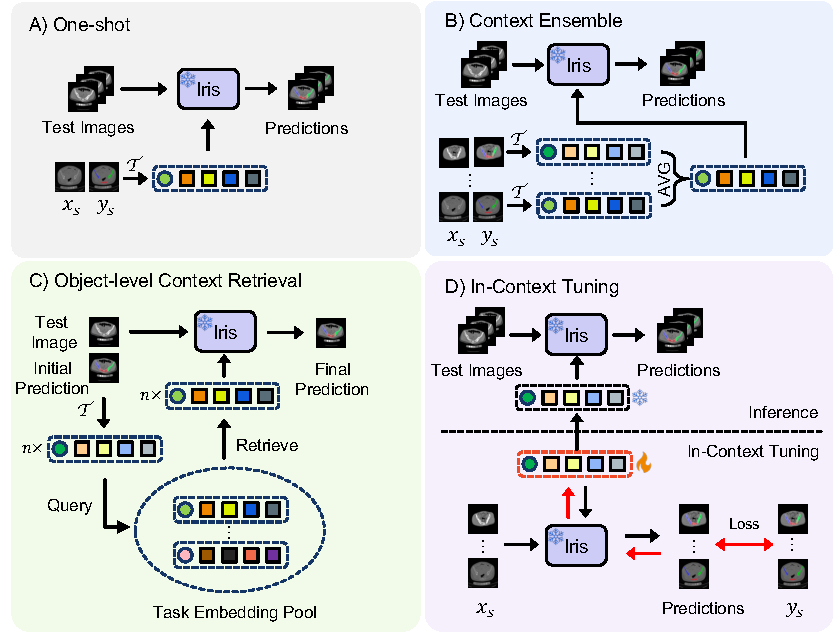
\includegraphics[width=\columnwidth]{./fig/inference_strategy.pdf}
\end{center}
\vspace{-1em}
\caption{Iris's flexible inference strategies. The red arrows indicates gradient backpropagation.}
\label{fig:inference_strategy}
\vspace{-1em}
\end{figure}





\begin{table*}[t]
\centering
\caption{Comparison of segmentation performance across different in-distribution datasets. Values represent mean Dice scores (\%).}
\label{tab:id_results}
%\definecolor{lightgray}{rgb}{0.92, 0.92, 0.92}
\resizebox{\textwidth}{!}{
\begin{tabular}{l|cccccccccccc|c}
\toprule
\multirow{2}{*}{Method} & \multicolumn{12}{c|}{Dataset} & \multirow{2}{*}{AVG} \\
\cline{2-13}
& AMOS & AMOS & Auto & BCV & Brain & CHAOS & KiTS & LiTS & MnM & StructSeg & StructSeg & CSI-Wat & \\
& CT & MR & PET & & & & Tumor &Tumor & & H\&N & Tho & & \\
\midrule
\multicolumn{14}{l}{\textit{Task-specific Model (Upper Bound)}} \\
nnUNet & 88.67 & 85.42 & 67.21 & 83.38 & 94.12 & 91.13 & 81.72 & 63.11 & 85.59 & 78.17 & 88.53 & 91.11 & 83.18 \\
\midrule
\multicolumn{14}{l}{\textit{Multi-task Universal Model (Upper Bound)}} \\
Clip-driven & 88.95 & 86.41 & 70.01 & 85.03 & 95.06 & 91.71 & 82.73 & 65.43 & 86.12 & 78.44 & 89.27 & 90.98 & 84.18 \\
UniSeg & 89.11 & 86.58 & 70.09 & 85.42 & 95.29 & 91.83 & 82.99 & 65.87 & 86.29 & 78.72 & 89.42 & 91.23 & 84.40 \\
Multi-Talent & 89.15 & 86.58 & 70.89 & 85.20 & 95.77 & 91.38 & 82.32 & 65.53 & 86.30 & 80.09 & 89.09 & 91.32 & 84.47 \\
\midrule
\multicolumn{14}{l}{\textit{Positional Prompt}} \\
SAM & 22.23 & 17.82 & 20.10 & 23.34 & 20.51 & 20.01 & 18.21 & 12.08 & 10.23 & 17.23 & 24.81 & 13.20 & 17.97 \\
SAM-Med 2D & 50.12 & 48.66 & 38.03 & 50.32 & 35.28 & 50.32 & 30.23 & 23.27 & 40.33 & 39.32 & 63.87 & 34.87 & 40.58 \\
SAM-Med 3D & 79.19 & 76.18 & 67.14 & 79.89 & 42.29 & 84.79 & 79.32 & 32.93 & 52.67 & 68.83 & 83.56 & 74.23 & 68.42 \\
\midrule
\multicolumn{14}{l}{\textit{In-Context}} \\
SegGPT & 45.37 & 51.78 & 48.29 & 49.78 & 85.27 & 63.72 & 40.78 & 35.98 & 74.12 & 40.28 & 67.28 & 85.59 & 57.35 \\
UniverSeg & 57.24 & 52.43 & 47.23 & 45.26 & 87.76 & 60.46 & 45.72 & 36.21 & 75.24 & 42.98 & 66.95 & 86.68 & 58.68 \\
Tyche-IS & 59.57 & 54.78 & 50.98 & 47.67 & 89.28 & 62.73 & 49.27 & 37.02 & 78.92 & 45.33 & 69.89 & 88.99 & 61.20 \\
\rowcolor{lightgray} Iris (ours) & 89.56 & 86.70 & 70.02 & 85.73 & 96.04 & 91.85 & 81.54 & 65.02 & 86.08 & 80.36 & 89.42 & 91.97 & 84.52 \\
\bottomrule
\end{tabular}
}
\vspace{-1em}
\end{table*}


\subsection{Flexible Inference Strategies}
After training, Iris supports multiple inference strategies suitable for different practical scenarios (see in Figure~\ref{fig:inference_strategy}).


\noindent\textbf{Efficient one-shot inference.} With just one reference example, Iris first encodes the task into compact embeddings $\boldsymbol{T}$ that can be stored and reused across multiple query images. Unlike major in-context learning methods to recompute contextual information for each query image, our design greatly eliminates redundant computation. Moreover, Iris can segment multiple classes in a single forward pass, contrasting with methods (e.g., UniverSeg~\cite{butoi2023universeg}) that require separate passes per class. The minimal storage requirement of these embeddings makes Iris particularly desirable for large-scale data processing pipelines.


\noindent\textbf{Context ensemble.}
For tasks with multiple reference examples, Iris supports context ensemble for improving performance. We compute task embeddings for each example and average them to create a more robust task representation. This simple averaging strategy combines information from multiple references while maintaining computational efficiency. We extent context ensemble for classes seen during training. Specifically, we maintain a class-specific memory bank that continuously updates task embeddings through exponential moving average (EMA) during the training process. This memory bank stores representative task embeddings for each seen class, enabling direct segmentation for seen classes during inference without requiring context encoding.


\noindent\textbf{Object-level context retrieval.} For multi-class segmentation with a pool of reference examples, conventional approaches typically employ image-level retrieval using global embeddings to select semantically similar references~\cite{zhang2023makes}. However, this strategy is suboptimal for medical images where multiple anatomical structures coexist, as global embeddings average features across all structures. To enable more precise reference selection, we propose an object-level (class-level) context retrieval strategy. Our approach first encodes class-specific task embeddings for each reference example through our task encoding module - for a reference image with $n$ anatomical classes, we encode $n$ separate task embeddings. For a query image, we obtain initial object segmentation masks using task embeddings from a randomly selected reference. These initial masks are then used to encode $n$ class-specific query task embeddings, which are compared with corresponding reference embeddings in the pool using cosine similarity to select the most similar reference for each class independently. This fine-grained matching allows different structures within the same query image to find their most appropriate references, leading to more accurate segmentation compared to image-level approaches.



\noindent\textbf{In-context tuning.} For scenarios requiring adaptation without a full model fine-tuning, Iris offers a lightweight tuning strategy by optimizing only the task embeddings while keeping the model parameters fixed. This tuning process minimizes the segmentation loss between model predictions and ground truth by updating the task embeddings through the gradient descent. In particular, the optimized embeddings can then be stored and reused for similar cases, offering a practical balance between adaptation capability and computational efficiency.



